% Options for packages loaded elsewhere
\PassOptionsToPackage{unicode}{hyperref}
\PassOptionsToPackage{hyphens}{url}
%
\documentclass[
]{article}
\usepackage{lmodern}
\usepackage{amssymb,amsmath}
\usepackage{ifxetex,ifluatex}
\ifnum 0\ifxetex 1\fi\ifluatex 1\fi=0 % if pdftex
  \usepackage[T1]{fontenc}
  \usepackage[utf8]{inputenc}
  \usepackage{textcomp} % provide euro and other symbols
\else % if luatex or xetex
  \usepackage{unicode-math}
  \defaultfontfeatures{Scale=MatchLowercase}
  \defaultfontfeatures[\rmfamily]{Ligatures=TeX,Scale=1}
\fi
% Use upquote if available, for straight quotes in verbatim environments
\IfFileExists{upquote.sty}{\usepackage{upquote}}{}
\IfFileExists{microtype.sty}{% use microtype if available
  \usepackage[]{microtype}
  \UseMicrotypeSet[protrusion]{basicmath} % disable protrusion for tt fonts
}{}
\makeatletter
\@ifundefined{KOMAClassName}{% if non-KOMA class
  \IfFileExists{parskip.sty}{%
    \usepackage{parskip}
  }{% else
    \setlength{\parindent}{0pt}
    \setlength{\parskip}{6pt plus 2pt minus 1pt}}
}{% if KOMA class
  \KOMAoptions{parskip=half}}
\makeatother
\usepackage{xcolor}
\IfFileExists{xurl.sty}{\usepackage{xurl}}{} % add URL line breaks if available
\IfFileExists{bookmark.sty}{\usepackage{bookmark}}{\usepackage{hyperref}}
\hypersetup{
  pdftitle={Supplementary Material for `Effects of long-term use of cover crops on weed seedbanks'},
  pdfauthor={Nichols et al.~2020},
  hidelinks,
  pdfcreator={LaTeX via pandoc}}
\urlstyle{same} % disable monospaced font for URLs
\usepackage[margin=1in]{geometry}
\usepackage{graphicx,grffile}
\makeatletter
\def\maxwidth{\ifdim\Gin@nat@width>\linewidth\linewidth\else\Gin@nat@width\fi}
\def\maxheight{\ifdim\Gin@nat@height>\textheight\textheight\else\Gin@nat@height\fi}
\makeatother
% Scale images if necessary, so that they will not overflow the page
% margins by default, and it is still possible to overwrite the defaults
% using explicit options in \includegraphics[width, height, ...]{}
\setkeys{Gin}{width=\maxwidth,height=\maxheight,keepaspectratio}
% Set default figure placement to htbp
\makeatletter
\def\fps@figure{htbp}
\makeatother
\setlength{\emergencystretch}{3em} % prevent overfull lines
\providecommand{\tightlist}{%
  \setlength{\itemsep}{0pt}\setlength{\parskip}{0pt}}
\setcounter{secnumdepth}{-\maxdimen} % remove section numbering
\usepackage{float}
\floatplacement{figure}{H}
\usepackage{booktabs}
\usepackage{longtable}
\usepackage{array}
\usepackage{multirow}
\usepackage{wrapfig}
\usepackage{float}
\usepackage{colortbl}
\usepackage{pdflscape}
\usepackage{tabu}
\usepackage{threeparttable}
\usepackage{threeparttablex}
\usepackage[normalem]{ulem}
\usepackage{makecell}

\title{Supplementary Material for `Effects of long-term use of cover crops on
weed seedbanks'}
\author{Nichols et al.~2020}
\date{7/15/2020}

\begin{document}
\maketitle

\hypertarget{general-site-management-summary}{%
\section{General Site Management
Summary}\label{general-site-management-summary}}

\begin{table}[H]

\caption{\label{tab:gentbl}General Site Description}
\centering
\begin{tabular}[t]{>{\centering\arraybackslash}p{5em}>{\centering\arraybackslash}p{5em}>{\centering\arraybackslash}p{5em}>{\centering\arraybackslash}p{3em}>{\centering\arraybackslash}p{3em}>{\centering\arraybackslash}p{3em}c}
\toprule
Site Description & General Location & Treatment Description & Year of Initiation & Crop Planted in 2019 & Number of Treatment Replicates & Sampled in 2019\\
\midrule
\cellcolor{gray!6}{} & \cellcolor{gray!6}{Boyd Farm, Boone, field 44} & \cellcolor{gray!6}{maize/soybean grain rotation, with and without rye cover crop} & \cellcolor{gray!6}{2009} & \cellcolor{gray!6}{maize} & \cellcolor{gray!6}{5} & \cellcolor{gray!6}{Y}\\

\multirow{-2}{*}{\centering\arraybackslash Central Grain} & Boyd Farm, Boone, field 42 & maize/soybean grain rotation, with and without rye cover crop & 2009 & soy & 5 & Y\\
\cmidrule{1-7}
\cellcolor{gray!6}{} & \cellcolor{gray!6}{Boyd Farm, Boone, field 44} & \cellcolor{gray!6}{maize silage/soybean grain rotation, with and without rye cover crop} & \cellcolor{gray!6}{2002} & \cellcolor{gray!6}{maize silage} & \cellcolor{gray!6}{5} & \cellcolor{gray!6}{Y}\\

\multirow{-2}{*}{\centering\arraybackslash Central Silage} & Boyd Farm, Boone, field 42 & maize silage/soybean grain rotation, with and without rye cover crop & 2002 & soy & 5 & N\\
\cmidrule{1-7}
\cellcolor{gray!6}{West} & \cellcolor{gray!6}{Jefferson, IA} & \cellcolor{gray!6}{maize/soybean grain rotation, with and without rye cover crop} & \cellcolor{gray!6}{2008} & \cellcolor{gray!6}{maize} & \cellcolor{gray!6}{4} & \cellcolor{gray!6}{Y}\\
\cmidrule{1-7}
East & Washington, IA & maize/soybean grain rotation, with and without rye cover crop & 2009 & soybeans & 4 & Y\\
\bottomrule
\end{tabular}
\end{table}

\newpage

\begin{table}[H]

\caption{\label{tab:herbtable}2018-2019 Herbicide Use}
\centering
\begin{tabular}[t]{>{\centering\arraybackslash}p{8em}>{\centering\arraybackslash}p{8em}>{\centering\arraybackslash}p{8em}>{\centering\arraybackslash}p{8em}}
\toprule
Site Description & Herbicides Used in 2018 Growing Season & Herbicdes Used in Fall 2018 & Herbicides Used in Spring 2019\\
\midrule
\cellcolor{gray!6}{Central Grain} & \cellcolor{gray!6}{glyphosate 1 week before soybean planting} & \cellcolor{gray!6}{none} & \cellcolor{gray!6}{glyphosate 1 week before maize planting; metalochlor, atrazine, and mesotrione at planting}\\
\multirow{-2}{8em}{\centering\arraybackslash Central Grain} & glyphosate 1 week before maize planting; metalochlor, atrazine, and mesotrione at planting & none & glyphosate 1 week before soybean planting\\
\cmidrule{1-4}
\cellcolor{gray!6}{Central Silage} & \cellcolor{gray!6}{glyphosate 1 week before soybean planting} & \cellcolor{gray!6}{none} & \cellcolor{gray!6}{glyphosate 1 week before maize planting; metalochlor, atrazine, and mesotrione at planting}\\
\multirow{-2}{8em}{\centering\arraybackslash Central Silage} & glyphosate 1 week before maize planting; metalochlor, atrazine, and mesotrione at planting & none & glyphosate 1 week before soybean planting\\
\cmidrule{1-4}
\cellcolor{gray!6}{West} & \cellcolor{gray!6}{glyphosate before planting; glyphosate and fluthiacet-methyl at planting} & \cellcolor{gray!6}{none} & \cellcolor{gray!6}{glyphosate before planting; glyphosate and fluthiacet-methyl at planting}\\
East & glyphosate and acetochlor  before planting (April 15), atrazine, acetochlor at planting (May 14); acetochlor and glyphosate after planting (June 15) & none & chlorimuron-ethyl, flumioxazin, pyroxasulfone, and glyphosate before planting, dicamba and acetochlor after planting\\
\bottomrule
\end{tabular}
\end{table}

\newpage

\begin{table}[H]

\caption{\label{tab:mgmttable}General Management}
\centering
\begin{tabular}[t]{c>{\centering\arraybackslash}p{7em}>{\centering\arraybackslash}p{5em}>{\centering\arraybackslash}p{5em}>{\centering\arraybackslash}p{5em}>{\centering\arraybackslash}p{5em}>{\centering\arraybackslash}p{5em}}
\toprule
Site Description & General Herbicide Regime & General Date of Cover Crop Termination & General Date of Crop Planting & Inorganic Fertilizer Used & Organic Fertilizer Used & Tillage Used\\
\midrule
\cellcolor{gray!6}{Central Grain} & \cellcolor{gray!6}{burndown, residual herbicide at maize planting} & \cellcolor{gray!6}{15-Apr} & \cellcolor{gray!6}{26-Apr} & \cellcolor{gray!6}{Y} & \cellcolor{gray!6}{NA} & \cellcolor{gray!6}{N}\\
\multirow{-2}{*}{\centering\arraybackslash Central Grain} & burndown, residual herbicide at maize planting & 25-Apr & 5-May & Y & NA & N\\
\cmidrule{1-7}
\cellcolor{gray!6}{Central Silage} & \cellcolor{gray!6}{burndown, residual herbicide at maize planting} & \cellcolor{gray!6}{15-Apr} & \cellcolor{gray!6}{26-Apr} & \cellcolor{gray!6}{Y} & \cellcolor{gray!6}{NA} & \cellcolor{gray!6}{N}\\
\multirow{-2}{*}{\centering\arraybackslash Central Silage} & burndown, residual herbicide at maize planting & 25-Apr & 5-May & Y & NA & N\\
\cmidrule{1-7}
\cellcolor{gray!6}{West} & \cellcolor{gray!6}{burndown, pre-emergent herbicide} & \cellcolor{gray!6}{1-May} & \cellcolor{gray!6}{10-May} & \cellcolor{gray!6}{Y} & \cellcolor{gray!6}{chicken or turkey manure} & \cellcolor{gray!6}{N}\\
East & burndown, residual herbicide at planting, another application on maize at \textasciitilde{}V6 & 1-May & 5-May & Y & liquid swine, \textasciitilde{}3000 gal/ac every other year to entire field & N\\
\bottomrule
\end{tabular}
\end{table}

\newpage

\hypertarget{cover-crop-biomass-production-over-past-10-years-of-trials}{%
\section{Cover crop biomass production over past 10 years of
trials}\label{cover-crop-biomass-production-over-past-10-years-of-trials}}

\begin{figure}
\centering
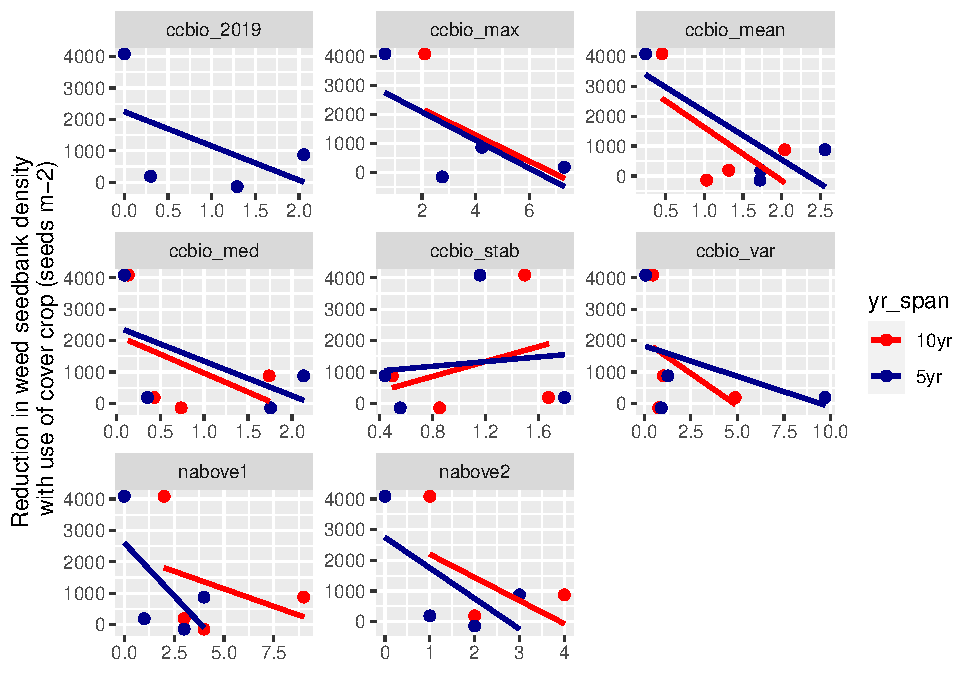
\includegraphics{supp-mat_files/figure-latex/unnamed-chunk-1-1.pdf}
\caption{Winter rye cover crop biomass production at each trial (inset
map, more information in Table 1) from 2010-2019 with solid lines
representing grain-based maize (Zea mays)-soybean (Glycine max) systems
and the dashed line the silage-based system.}
\end{figure}

\newpage

\hypertarget{field-wet-soil-amounts}{%
\section{Field wet soil amounts}\label{field-wet-soil-amounts}}

\begin{table}[H]

\caption{\label{tab:soilwgtstbl}Wet Soil Weights Immediately After Sampling}
\centering
\begin{tabular}[t]{ccccc}
\toprule
site & cc\_trt & rep & soilwt\_g & notes\\
\midrule
\cellcolor{gray!6}{BC} & \cellcolor{gray!6}{no} & \cellcolor{gray!6}{1} & \cellcolor{gray!6}{6718.3} & \cellcolor{gray!6}{sampled 4/8, 12-6pm}\\
 & rye & 1 & 6936.2 & sampled 4/8, 12-6pm\\

\cellcolor{gray!6}{BC} & \cellcolor{gray!6}{no} & \cellcolor{gray!6}{2} & \cellcolor{gray!6}{6838.6} & \cellcolor{gray!6}{sampled 4/8, 12-6pm}\\
 & rye & 2 & 5965.2 & sampled 4/8, 12-6pm\\

\cellcolor{gray!6}{BC} & \cellcolor{gray!6}{no} & \cellcolor{gray!6}{3} & \cellcolor{gray!6}{6260.4} & \cellcolor{gray!6}{sampled 4/8, 12-6pm}\\
 & rye & 3 & 6136.0 & sampled 4/8, 12-6pm\\

\cellcolor{gray!6}{BC} & \cellcolor{gray!6}{no} & \cellcolor{gray!6}{4} & \cellcolor{gray!6}{5554.9} & \cellcolor{gray!6}{sampled 4/9}\\
 & rye & 4 & 6312.7 & sampled 4/9\\

\cellcolor{gray!6}{BC} & \cellcolor{gray!6}{no} & \cellcolor{gray!6}{5} & \cellcolor{gray!6}{5866.2} & \cellcolor{gray!6}{sampled 4/9}\\
\multirow[t]{-10}{*}{\centering\arraybackslash BC} & rye & 5 & 5981.1 & sampled 4/9\\
\cmidrule{1-5}
\cellcolor{gray!6}{Bcsil} & \cellcolor{gray!6}{rye} & \cellcolor{gray!6}{1} & \cellcolor{gray!6}{6340.0} & \cellcolor{gray!6}{sampled 4/16, 2-6pm}\\
 & no & 1 & 5800.0 & sampled 4/16, 2-6pm\\

\cellcolor{gray!6}{Bcsil} & \cellcolor{gray!6}{rye} & \cellcolor{gray!6}{2} & \cellcolor{gray!6}{5990.0} & \cellcolor{gray!6}{sampled 4/16, 2-6pm}\\
 & no & 2 & 6100.0 & sampled 4/16, 2-6pm\\

\cellcolor{gray!6}{Bcsil} & \cellcolor{gray!6}{no} & \cellcolor{gray!6}{3} & \cellcolor{gray!6}{6245.5} & \cellcolor{gray!6}{sampled 4/8}\\
 & rye & 3 & 6160.2 & sampled 4/8\\

\cellcolor{gray!6}{Bcsil} & \cellcolor{gray!6}{no} & \cellcolor{gray!6}{4} & \cellcolor{gray!6}{6240.2} & \cellcolor{gray!6}{sampled 4/8}\\
 & rye & 4 & 6007.5 & sampled 4/8\\

\cellcolor{gray!6}{Bcsil} & \cellcolor{gray!6}{no} & \cellcolor{gray!6}{5} & \cellcolor{gray!6}{6682.9} & \cellcolor{gray!6}{sampled 4/8}\\
\multirow[t]{-10}{*}{\centering\arraybackslash Bcsil} & rye & 5 & 6045.7 & sampled 4/8\\
\cmidrule{1-5}
\cellcolor{gray!6}{BS} & \cellcolor{gray!6}{rye} & \cellcolor{gray!6}{1} & \cellcolor{gray!6}{6068.7} & \cellcolor{gray!6}{sampled 4/9}\\
 & no & 2 & 6240.3 & sampled 4/9\\

\cellcolor{gray!6}{BS} & \cellcolor{gray!6}{rye} & \cellcolor{gray!6}{2} & \cellcolor{gray!6}{5950.5} & \cellcolor{gray!6}{sampled 4/9}\\
 & no & 3 & 5885.7 & sampled 4/9\\

\cellcolor{gray!6}{BS} & \cellcolor{gray!6}{rye} & \cellcolor{gray!6}{3} & \cellcolor{gray!6}{5734.1} & \cellcolor{gray!6}{sampled 4/9}\\
 & no & 4 & 6213.3 & sampled 4/9\\

\cellcolor{gray!6}{BS} & \cellcolor{gray!6}{rye} & \cellcolor{gray!6}{4} & \cellcolor{gray!6}{5968.2} & \cellcolor{gray!6}{sampled 4/9}\\
 & no & 5 & 6175.8 & sampled 4/9\\

\cellcolor{gray!6}{BS} & \cellcolor{gray!6}{rye} & \cellcolor{gray!6}{5} & \cellcolor{gray!6}{6050.4} & \cellcolor{gray!6}{sampled 4/9}\\
 & no & 1 & 5349.6 & sampled 4/6, 8-5pm\\

\cellcolor{gray!6}{East} & \cellcolor{gray!6}{rye} & \cellcolor{gray!6}{1} & \cellcolor{gray!6}{5460.6} & \cellcolor{gray!6}{sampled 4/6, 8-5pm}\\
 & no & 2 & 5235.5 & sampled 4/6, 8-5pm\\

\cellcolor{gray!6}{East} & \cellcolor{gray!6}{rye} & \cellcolor{gray!6}{2} & \cellcolor{gray!6}{5055.2} & \cellcolor{gray!6}{sampled 4/6, 8-5pm}\\
 & no & 3 & 5211.1 & sampled 4/6, 8-5pm\\

\cellcolor{gray!6}{East} & \cellcolor{gray!6}{rye} & \cellcolor{gray!6}{3} & \cellcolor{gray!6}{4991.7} & \cellcolor{gray!6}{sampled 4/6, 8-5pm}\\
 & no & 4 & 5401.6 & sampled 4/6, 8-5pm\\

\cellcolor{gray!6}{East} & \cellcolor{gray!6}{rye} & \cellcolor{gray!6}{4} & \cellcolor{gray!6}{5163.9} & \cellcolor{gray!6}{sampled 4/6, 8-5pm}\\
 & no & 1 & 6314.0 & sampled 4/17, 9-2pm\\

\cellcolor{gray!6}{West} & \cellcolor{gray!6}{rye} & \cellcolor{gray!6}{1} & \cellcolor{gray!6}{6401.0} & \cellcolor{gray!6}{sampled 4/17, 9-2pm}\\
 & no & 2 & 5841.0 & sampled 4/17, 9-2pm\\

\cellcolor{gray!6}{West} & \cellcolor{gray!6}{rye} & \cellcolor{gray!6}{2} & \cellcolor{gray!6}{5543.0} & \cellcolor{gray!6}{sampled 4/17, 9-2pm}\\
 & no & 3 & 5698.0 & sampled 4/17, 9-2pm\\

\cellcolor{gray!6}{West} & \cellcolor{gray!6}{rye} & \cellcolor{gray!6}{3} & \cellcolor{gray!6}{5947.0} & \cellcolor{gray!6}{sampled 4/17, 9-2pm}\\
 & no & 4 & 6057.0 & sampled 4/17, 9-2pm\\

\cellcolor{gray!6}{West} & \cellcolor{gray!6}{rye} & \cellcolor{gray!6}{4} & \cellcolor{gray!6}{5989.0} & \cellcolor{gray!6}{sampled 4/17, 9-2pm}\\
\bottomrule
\end{tabular}
\end{table}

\newpage

\hypertarget{statistical-results}{%
\section{Statistical Results}\label{statistical-results}}

\hypertarget{linear-models-on-seedbank-density}{%
\subsection{Linear models on seedbank
density}\label{linear-models-on-seedbank-density}}

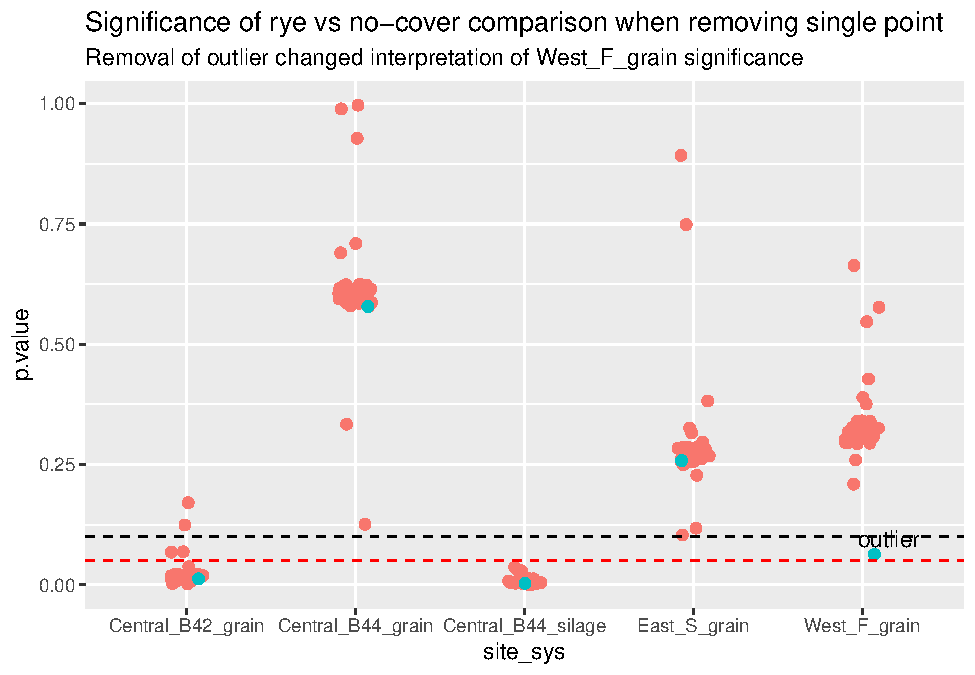
\includegraphics{supp-mat_files/figure-latex/loo-1.pdf}

Values are presented for the models run with the full dataset (XX\_full)
and with the outlier removed (XX\_out-rm)

\begin{table}[H]

\caption{\label{tab:contrasts}Contrasts using full dataset (full) and dataset with outlier removed (out-rm)}
\centering
\begin{tabular}[t]{cccccccc}
\toprule
model & site\_sys & level1 & level2 & estimate & std.error & z.ratio & p.value\\
\midrule
\cellcolor{gray!6}{pois\_out-rm} & \cellcolor{gray!6}{Central\_B42\_grain} & \cellcolor{gray!6}{no} & \cellcolor{gray!6}{rye} & \cellcolor{gray!6}{-0.85} & \cellcolor{gray!6}{0.34} & \cellcolor{gray!6}{-2.50} & \cellcolor{gray!6}{0.01}\\
 & Central\_B44\_grain & no & rye & 0.18 & 0.33 & 0.56 & 0.58\\

\cellcolor{gray!6}{pois\_out-rm} & \cellcolor{gray!6}{Central\_B44\_silage} & \cellcolor{gray!6}{no} & \cellcolor{gray!6}{rye} & \cellcolor{gray!6}{0.95} & \cellcolor{gray!6}{0.32} & \cellcolor{gray!6}{2.96} & \cellcolor{gray!6}{0.00}\\
 & East\_S\_grain & no & rye & 0.42 & 0.38 & 1.13 & 0.26\\

\cellcolor{gray!6}{pois\_out-rm} & \cellcolor{gray!6}{West\_F\_grain} & \cellcolor{gray!6}{no} & \cellcolor{gray!6}{rye} & \cellcolor{gray!6}{0.71} & \cellcolor{gray!6}{0.38} & \cellcolor{gray!6}{1.86} & \cellcolor{gray!6}{0.06}\\
 & Central\_B42\_grain & no & rye & -0.85 & 0.35 & -2.39 & 0.02\\

\cellcolor{gray!6}{pois\_full} & \cellcolor{gray!6}{Central\_B44\_grain} & \cellcolor{gray!6}{no} & \cellcolor{gray!6}{rye} & \cellcolor{gray!6}{0.18} & \cellcolor{gray!6}{0.34} & \cellcolor{gray!6}{0.52} & \cellcolor{gray!6}{0.60}\\
 & Central\_B44\_silage & no & rye & 0.95 & 0.33 & 2.83 & 0.00\\

\cellcolor{gray!6}{pois\_full} & \cellcolor{gray!6}{East\_S\_grain} & \cellcolor{gray!6}{no} & \cellcolor{gray!6}{rye} & \cellcolor{gray!6}{0.43} & \cellcolor{gray!6}{0.39} & \cellcolor{gray!6}{1.09} & \cellcolor{gray!6}{0.28}\\
\multirow{-5}{*}{\centering\arraybackslash pois\_full} & West\_F\_grain & no & rye & 0.36 & 0.36 & 1.00 & 0.32\\
\cmidrule{1-8}
\cellcolor{gray!6}{binom\_out-rm} & \cellcolor{gray!6}{Central\_B42\_grain} & \cellcolor{gray!6}{no} & \cellcolor{gray!6}{rye} & \cellcolor{gray!6}{-0.97} & \cellcolor{gray!6}{0.34} & \cellcolor{gray!6}{-2.88} & \cellcolor{gray!6}{0.00}\\
 & Central\_B44\_grain & no & rye & 0.24 & 0.32 & 0.75 & 0.45\\

\cellcolor{gray!6}{binom\_out-rm} & \cellcolor{gray!6}{Central\_B44\_silage} & \cellcolor{gray!6}{no} & \cellcolor{gray!6}{rye} & \cellcolor{gray!6}{1.01} & \cellcolor{gray!6}{0.31} & \cellcolor{gray!6}{3.24} & \cellcolor{gray!6}{0.00}\\
 & East\_S\_grain & no & rye & 0.44 & 0.36 & 1.22 & 0.22\\

\cellcolor{gray!6}{binom\_out-rm} & \cellcolor{gray!6}{West\_F\_grain} & \cellcolor{gray!6}{no} & \cellcolor{gray!6}{rye} & \cellcolor{gray!6}{0.71} & \cellcolor{gray!6}{0.37} & \cellcolor{gray!6}{1.89} & \cellcolor{gray!6}{0.06}\\
 & Central\_B42\_grain & no & rye & -0.98 & 0.36 & -2.69 & 0.01\\

\cellcolor{gray!6}{binom\_full} & \cellcolor{gray!6}{Central\_B44\_grain} & \cellcolor{gray!6}{no} & \cellcolor{gray!6}{rye} & \cellcolor{gray!6}{0.24} & \cellcolor{gray!6}{0.35} & \cellcolor{gray!6}{0.70} & \cellcolor{gray!6}{0.49}\\
 & Central\_B44\_silage & no & rye & 1.01 & 0.34 & 3.00 & 0.00\\

\cellcolor{gray!6}{binom\_full} & \cellcolor{gray!6}{East\_S\_grain} & \cellcolor{gray!6}{no} & \cellcolor{gray!6}{rye} & \cellcolor{gray!6}{0.44} & \cellcolor{gray!6}{0.39} & \cellcolor{gray!6}{1.14} & \cellcolor{gray!6}{0.26}\\
\multirow{-5}{*}{\centering\arraybackslash binom\_full} & West\_F\_grain & no & rye & 0.28 & 0.37 & 0.74 & 0.46\\
\bottomrule
\end{tabular}
\end{table}

\begin{table}[H]

\caption{\label{tab:estimates}Estimates using full dataset (full) and dataset with outlier removed (out-rm)}
\centering
\begin{tabular}[t]{ccccccc}
\toprule
model & site\_sys & cc\_trt & estimate & std.error & asymp.LCL & asymp.UCL\\
\midrule
\cellcolor{gray!6}{pois\_out-rm} & \cellcolor{gray!6}{Central\_B42\_grain} & \cellcolor{gray!6}{no} & \cellcolor{gray!6}{2.59} & \cellcolor{gray!6}{0.32} & \cellcolor{gray!6}{1.97} & \cellcolor{gray!6}{3.21}\\
 & \multirow{-2}{*}{\centering\arraybackslash Central\_B42\_grain} & rye & 3.44 & 0.31 & 2.84 & 4.05\\

\cellcolor{gray!6}{pois\_out-rm} & \cellcolor{gray!6}{Central\_B44\_grain} & \cellcolor{gray!6}{no} & \cellcolor{gray!6}{3.33} & \cellcolor{gray!6}{0.31} & \cellcolor{gray!6}{2.73} & \cellcolor{gray!6}{3.93}\\
 & \multirow{-2}{*}{\centering\arraybackslash Central\_B44\_grain} & rye & 3.15 & 0.31 & 2.55 & 3.75\\

\cellcolor{gray!6}{pois\_out-rm} & \cellcolor{gray!6}{Central\_B44\_silage} & \cellcolor{gray!6}{no} & \cellcolor{gray!6}{4.35} & \cellcolor{gray!6}{0.30} & \cellcolor{gray!6}{3.77} & \cellcolor{gray!6}{4.94}\\
 & \multirow{-2}{*}{\centering\arraybackslash Central\_B44\_silage} & rye & 3.41 & 0.30 & 2.81 & 4.01\\

\cellcolor{gray!6}{pois\_out-rm} & \cellcolor{gray!6}{East\_S\_grain} & \cellcolor{gray!6}{no} & \cellcolor{gray!6}{3.33} & \cellcolor{gray!6}{0.34} & \cellcolor{gray!6}{2.65} & \cellcolor{gray!6}{4.00}\\
 & \multirow{-2}{*}{\centering\arraybackslash East\_S\_grain} & rye & 2.90 & 0.35 & 2.21 & 3.59\\

\cellcolor{gray!6}{pois\_out-rm} & \cellcolor{gray!6}{West\_F\_grain} & \cellcolor{gray!6}{no} & \cellcolor{gray!6}{6.02} & \cellcolor{gray!6}{0.33} & \cellcolor{gray!6}{5.38} & \cellcolor{gray!6}{6.66}\\
\multirow{-10}{*}{\centering\arraybackslash pois\_out-rm} & \multirow{-2}{*}{\centering\arraybackslash West\_F\_grain} & rye & 5.31 & 0.37 & 4.59 & 6.04\\
\cmidrule{1-7}
\cellcolor{gray!6}{pois\_full} & \cellcolor{gray!6}{Central\_B42\_grain} & \cellcolor{gray!6}{no} & \cellcolor{gray!6}{2.59} & \cellcolor{gray!6}{0.33} & \cellcolor{gray!6}{1.94} & \cellcolor{gray!6}{3.24}\\
 & \multirow{-2}{*}{\centering\arraybackslash Central\_B42\_grain} & rye & 3.44 & 0.32 & 2.81 & 4.06\\

\cellcolor{gray!6}{pois\_full} & \cellcolor{gray!6}{Central\_B44\_grain} & \cellcolor{gray!6}{no} & \cellcolor{gray!6}{3.33} & \cellcolor{gray!6}{0.32} & \cellcolor{gray!6}{2.70} & \cellcolor{gray!6}{3.95}\\
 & \multirow{-2}{*}{\centering\arraybackslash Central\_B44\_grain} & rye & 3.15 & 0.32 & 2.52 & 3.77\\

\cellcolor{gray!6}{pois\_full} & \cellcolor{gray!6}{Central\_B44\_silage} & \cellcolor{gray!6}{no} & \cellcolor{gray!6}{4.35} & \cellcolor{gray!6}{0.31} & \cellcolor{gray!6}{3.74} & \cellcolor{gray!6}{4.96}\\
 & \multirow{-2}{*}{\centering\arraybackslash Central\_B44\_silage} & rye & 3.41 & 0.32 & 2.79 & 4.03\\

\cellcolor{gray!6}{pois\_full} & \cellcolor{gray!6}{East\_S\_grain} & \cellcolor{gray!6}{no} & \cellcolor{gray!6}{3.32} & \cellcolor{gray!6}{0.36} & \cellcolor{gray!6}{2.62} & \cellcolor{gray!6}{4.02}\\
 & \multirow{-2}{*}{\centering\arraybackslash East\_S\_grain} & rye & 2.90 & 0.36 & 2.18 & 3.61\\

\cellcolor{gray!6}{pois\_full} & \cellcolor{gray!6}{West\_F\_grain} & \cellcolor{gray!6}{no} & \cellcolor{gray!6}{6.02} & \cellcolor{gray!6}{0.34} & \cellcolor{gray!6}{5.35} & \cellcolor{gray!6}{6.69}\\
\multirow{-10}{*}{\centering\arraybackslash pois\_full} & \multirow{-2}{*}{\centering\arraybackslash West\_F\_grain} & rye & 5.66 & 0.34 & 4.99 & 6.33\\
\cmidrule{1-7}
\cellcolor{gray!6}{binom\_out-rm} & \cellcolor{gray!6}{Central\_B42\_grain} & \cellcolor{gray!6}{no} & \cellcolor{gray!6}{2.65} & \cellcolor{gray!6}{0.31} & \cellcolor{gray!6}{2.04} & \cellcolor{gray!6}{3.25}\\
 & \multirow{-2}{*}{\centering\arraybackslash Central\_B42\_grain} & rye & 3.62 & 0.30 & 3.02 & 4.21\\

\cellcolor{gray!6}{binom\_out-rm} & \cellcolor{gray!6}{Central\_B44\_grain} & \cellcolor{gray!6}{no} & \cellcolor{gray!6}{3.45} & \cellcolor{gray!6}{0.29} & \cellcolor{gray!6}{2.88} & \cellcolor{gray!6}{4.03}\\
 & \multirow{-2}{*}{\centering\arraybackslash Central\_B44\_grain} & rye & 3.21 & 0.30 & 2.63 & 3.79\\

\cellcolor{gray!6}{binom\_out-rm} & \cellcolor{gray!6}{Central\_B44\_silage} & \cellcolor{gray!6}{no} & \cellcolor{gray!6}{4.49} & \cellcolor{gray!6}{0.29} & \cellcolor{gray!6}{3.92} & \cellcolor{gray!6}{5.05}\\
 & \multirow{-2}{*}{\centering\arraybackslash Central\_B44\_silage} & rye & 3.47 & 0.29 & 2.90 & 4.05\\

\cellcolor{gray!6}{binom\_out-rm} & \cellcolor{gray!6}{East\_S\_grain} & \cellcolor{gray!6}{no} & \cellcolor{gray!6}{3.42} & \cellcolor{gray!6}{0.34} & \cellcolor{gray!6}{2.76} & \cellcolor{gray!6}{4.08}\\
 & \multirow{-2}{*}{\centering\arraybackslash East\_S\_grain} & rye & 2.98 & 0.34 & 2.31 & 3.64\\

\cellcolor{gray!6}{binom\_out-rm} & \cellcolor{gray!6}{West\_F\_grain} & \cellcolor{gray!6}{no} & \cellcolor{gray!6}{6.03} & \cellcolor{gray!6}{0.32} & \cellcolor{gray!6}{5.41} & \cellcolor{gray!6}{6.64}\\
\multirow{-10}{*}{\centering\arraybackslash binom\_out-rm} & \multirow{-2}{*}{\centering\arraybackslash West\_F\_grain} & rye & 5.32 & 0.36 & 4.62 & 6.02\\
\cmidrule{1-7}
\cellcolor{gray!6}{binom\_full} & \cellcolor{gray!6}{Central\_B42\_grain} & \cellcolor{gray!6}{no} & \cellcolor{gray!6}{2.65} & \cellcolor{gray!6}{0.32} & \cellcolor{gray!6}{2.01} & \cellcolor{gray!6}{3.28}\\
 & \multirow{-2}{*}{\centering\arraybackslash Central\_B42\_grain} & rye & 3.62 & 0.32 & 2.99 & 4.25\\

\cellcolor{gray!6}{binom\_full} & \cellcolor{gray!6}{Central\_B44\_grain} & \cellcolor{gray!6}{no} & \cellcolor{gray!6}{3.45} & \cellcolor{gray!6}{0.31} & \cellcolor{gray!6}{2.84} & \cellcolor{gray!6}{4.06}\\
 & \multirow{-2}{*}{\centering\arraybackslash Central\_B44\_grain} & rye & 3.21 & 0.31 & 2.60 & 3.82\\

\cellcolor{gray!6}{binom\_full} & \cellcolor{gray!6}{Central\_B44\_silage} & \cellcolor{gray!6}{no} & \cellcolor{gray!6}{4.49} & \cellcolor{gray!6}{0.31} & \cellcolor{gray!6}{3.89} & \cellcolor{gray!6}{5.09}\\
 & \multirow{-2}{*}{\centering\arraybackslash Central\_B44\_silage} & rye & 3.47 & 0.31 & 2.87 & 4.08\\

\cellcolor{gray!6}{binom\_full} & \cellcolor{gray!6}{East\_S\_grain} & \cellcolor{gray!6}{no} & \cellcolor{gray!6}{3.42} & \cellcolor{gray!6}{0.36} & \cellcolor{gray!6}{2.73} & \cellcolor{gray!6}{4.12}\\
 & \multirow{-2}{*}{\centering\arraybackslash East\_S\_grain} & rye & 2.98 & 0.36 & 2.28 & 3.68\\

\cellcolor{gray!6}{binom\_full} & \cellcolor{gray!6}{West\_F\_grain} & \cellcolor{gray!6}{no} & \cellcolor{gray!6}{6.04} & \cellcolor{gray!6}{0.33} & \cellcolor{gray!6}{5.38} & \cellcolor{gray!6}{6.69}\\
\multirow{-10}{*}{\centering\arraybackslash binom\_full} & \multirow{-2}{*}{\centering\arraybackslash West\_F\_grain} & rye & 5.76 & 0.34 & 5.09 & 6.43\\
\bottomrule
\end{tabular}
\end{table}

\hypertarget{biomass-metrics}{%
\subsection{Biomass metrics}\label{biomass-metrics}}

\begin{table}[H]

\caption{\label{tab:ccbio10yr}Cover crop biomass metrics, 10-year time frame}
\centering
\begin{tabular}[t]{ccccccccc}
\toprule
site\_sys & nabove1 & nabove2 & ccbio\_mean & ccbio\_med & ccbio\_var & ccbio\_max & ccbio\_stab & ccbio\_2019\\
\midrule
\cellcolor{gray!6}{Boyd\_grain} & \cellcolor{gray!6}{4} & \cellcolor{gray!6}{2} & \cellcolor{gray!6}{1.03} & \cellcolor{gray!6}{0.74} & \cellcolor{gray!6}{0.77} & \cellcolor{gray!6}{2.76} & \cellcolor{gray!6}{0.85} & \cellcolor{gray!6}{1.29}\\
Boyd\_silage & 9 & 4 & 2.04 & 1.74 & 1.02 & 4.23 & 0.50 & 2.05\\
\cmidrule{1-9}
\cellcolor{gray!6}{Funcke\_grain} & \cellcolor{gray!6}{2} & \cellcolor{gray!6}{1} & \cellcolor{gray!6}{0.45} & \cellcolor{gray!6}{0.14} & \cellcolor{gray!6}{0.46} & \cellcolor{gray!6}{2.11} & \cellcolor{gray!6}{1.50} & \cellcolor{gray!6}{0.00}\\
Stout\_grain & 3 & 2 & 1.32 & 0.43 & 4.89 & 7.30 & 1.68 & 0.30\\
\bottomrule
\end{tabular}
\end{table}

\begin{table}[H]

\caption{\label{tab:ccbio5yr}Cover crop biomass metrics, 5-year time frame}
\centering
\begin{tabular}[t]{ccccccccc}
\toprule
site\_sys & nabove1 & nabove2 & ccbio\_mean & ccbio\_med & ccbio\_var & ccbio\_max & ccbio\_stab & ccbio\_2019\\
\midrule
\cellcolor{gray!6}{Boyd\_grain} & \cellcolor{gray!6}{3} & \cellcolor{gray!6}{2} & \cellcolor{gray!6}{1.72} & \cellcolor{gray!6}{1.76} & \cellcolor{gray!6}{0.91} & \cellcolor{gray!6}{2.76} & \cellcolor{gray!6}{0.55} & \cellcolor{gray!6}{1.29}\\
Boyd\_silage & 4 & 3 & 2.56 & 2.13 & 1.27 & 4.23 & 0.44 & 2.05\\
\cmidrule{1-9}
\cellcolor{gray!6}{Funcke\_grain} & \cellcolor{gray!6}{0} & \cellcolor{gray!6}{0} & \cellcolor{gray!6}{0.24} & \cellcolor{gray!6}{0.09} & \cellcolor{gray!6}{0.08} & \cellcolor{gray!6}{0.63} & \cellcolor{gray!6}{1.16} & \cellcolor{gray!6}{0.00}\\
Stout\_grain & 1 & 1 & 1.73 & 0.36 & 9.71 & 7.30 & 1.80 & 0.30\\
\bottomrule
\end{tabular}
\end{table}

\begin{figure}
\centering
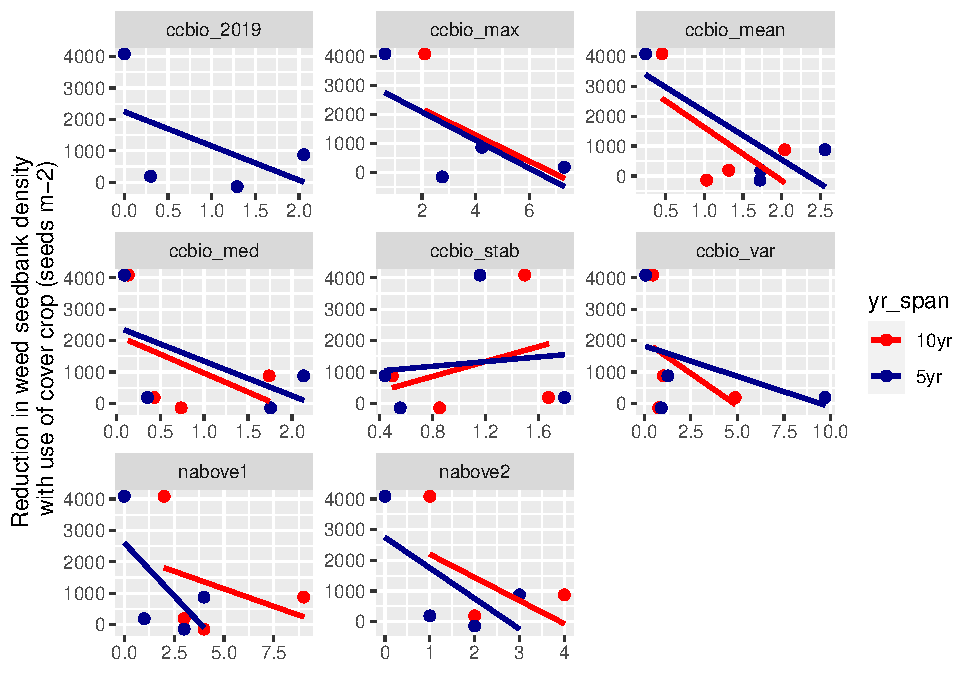
\includegraphics{supp-mat_files/figure-latex/unnamed-chunk-2-1.pdf}
\caption{Absolute change in seedbank density vs.~cover crop biomass
metrics}
\end{figure}

\begin{figure}
\centering
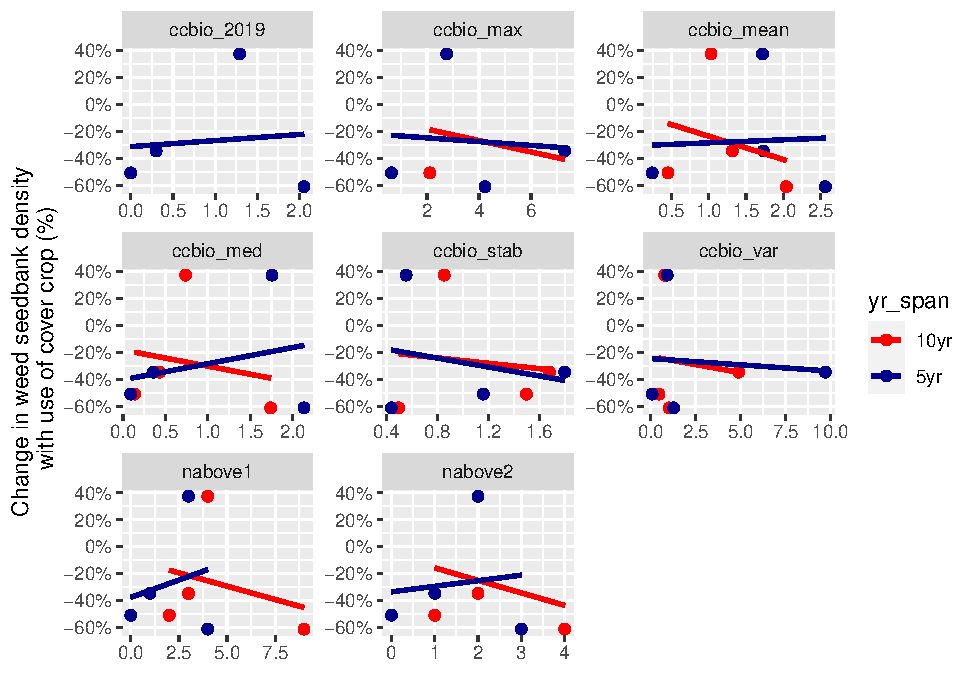
\includegraphics{supp-mat_files/figure-latex/unnamed-chunk-3-1.pdf}
\caption{Relative change in seedbank density vs.~cover crop biomass
metrics}
\end{figure}

\end{document}
